\section{Verifying  \lgname programs}
\label{sec:verification}

\newcommand{\Ev}{\ensuremath{e}\xspace}
\newcommand{\EvCond}{\ensuremath{\mathit{Cond}}\xspace}
\newcommand{\EvBody}{\ensuremath{\mathit{Body}}\xspace}

%\rg{round, program transition, event execution, $\delta$-transition are all defined at this point: program transition : events executed in some order, $\delta$-transition: simulataneous advancement of time, round = program + $\delta$-transition. }
% connect to definition of e.
%make the post definition on a set.

I have built the semantics of $\lgname$ in the \K framework to enable decoupled analyses of platform-independent discrete part and the platform-dependent (dynamic) parts of distributed multi-robot systems. The \emph{events} in an $\lgname$ program define the discrete computations in the system.
The effect of a robot $i$ executing event $\Ev \in \Event$ on a configuration $\gconfig \in \pwg$,
can be seen as a $\stmtrule$ application to  $\left\langle \gconfig.S, \gconfig.\lconfig{i}, \EvBody \right\rangle $,
where $\Ev$ is \emph{``eventName: {\normalfont\bf pre:} \EvCond\ {\normalfont\bf eff:} \EvBody''}.


\subsection{Reachable configurations}

Given a set of system configurations $\gset$,
we define the following functions using the semantic rules of \refsect{semantics}:
\begin{inparaenum}[(i)]
    \item $\Post_\Ev(\gconfig,i)$ returns the set of configurations obtained by robot $i$ executing event $\Ev \in \Event$ from a configuration $\gconfig$.
%          \sayan{are events deterministic? Did we discuss somewhere?}
    \item $\Post(\gset,i)$ returns the set of configurations obtained by robot $i$ executing any event from a configuration in $\gset$.
    \item $\Post(\gset,\pvec)$ returns all configurations visited, when robots execute their events in the order $\pvec$,
          where $\pvec$ is a sequence of $p_i \in \UINS$.
    \item $\Post(\gset)$ is the union of $\Post(\gset,\pvec)$ over all orders $\pvec$.
    \item $\Final(\gset)$ is the set of configurations reached from $\gset$ \emph{after} a program transition.
\end{inparaenum}

\begin{mdframed}
\footnotesize
\newcommand{\Skip}{\mathit{Skip}\xspace}
\begin{align*}
    \Post_\Ev(\gconfig,i) &:= \{ \gconfig' \mid \eec{\EvCond}{\gconfig.S, \gconfig.\lconfig{i}} \\
      & \ \ \ \ \ \ \land \left\langle \gconfig.S, \gconfig.\lconfig{i}, \EvBody \right\rangle \stmtrule \left\langle \gconfig'.S, \gconfig'.\lconfig{i}, \EndEvent \right\rangle\}, \\
    \Skip(\gconfig,i) &:= \{ \gconfig' \mid \left\langle \gconfig.S, \gconfig.\lconfig{i}, \EndEvent \right\rangle \stmtrule \left\langle \gconfig'.S, \gconfig'.\lconfig{i}, \EndEvent \right\rangle \} \\
    \Post(\gset,i) &:=  \bigcup_{\gconfig\in\gset} \left(\Skip(\gconfig, i) \cup \bigcup_{\Ev \in \Event} \Post_\Ev(\gconfig, i) \right),\\
    \Post(\gset,\pvec) &:= 
        \begin{cases}
            \emptyset, \text{ if } \pvec=()\\
            \Post(\Post(\gset,\pinit),\pvec'), \text{ if } \pvec=(\pinit, \pvec')\\
        \end{cases}\\
    \Post(\gset) &:=  \bigcup_{\pvec\in \mathit{perms}(\UINS)} \Post(\gset,\pvec), \\
    \Final(\gset) &:=  \left\{ \gconfig\in \Post(\gset)\mid \forall i \in \UINS, \gconfig.\lconfig{i}.\turn = \env \right\},
\end{align*}
\end{mdframed}
In the above, a sequence $\pvec=(\pinit, \pvec')$, is written  as a concatenation of the first element $\pinit$ and the suffix $\pvec'$.
Also, $\mathit{perms}(\UINS)$ refers to the set of permutations of $\UINS$.

Next, I define the configurations that are reached during and after an environment transition.
Recall that environment transitions capture the evolution of the actuator ports over a time interval $[0,\delta]$---all other parts of the configuration remain unchanged.
Our \lgname semantics defines the environment transitions with a \emph{parameter} which is a (possibly black-box) function that captures the dynamics of individual robots.%
\footnote{For different platforms, this function could be defined in closed form, as solutions of differential equations, or in terms of a numerical simulator.}
% 
Given such a function $f_i$ for each robot $i$,  we define the function $\traj: \pwg \times \left[0,\delta\right] \mapsto \pwg$ to represent the  evolution of the system over a  $[0,\delta]$ time interval.
$\traj$ is constructed by simply update all controller ports $\cp$ of all robots with their $f_i$.
That is,
\begin{small}
\[
\gconfig' = \traj(\gconfig, t) \Leftrightarrow
\left(
\begin{array}{l}
    \forall i \in \UINS, \gconfig'.\lconfig{i}.\cp = f_i(\gconfig.\lconfig{i}.\cp, t) \\
    \land\ \gconfig'.\lconfig{i}.M = \gconfig.\lconfig{i}.M \\
    \land\ \gconfig'.\lconfig{i}.\turn = \gconfig.\lconfig{i}.\turn\\
    \land\ \gconfig'.S = \gconfig.S \land \gconfig'.\tau = \gconfig.\tau \\
    \land\ \gconfig'.\turn = \gconfig.\turn \\
\end{array}
\right)
\]
\end{small}%
Notice those additional constraints making sure all other fields of $\gconfig$ and $\gconfig'$ stay the same.
The notaiton $\land \dots$ is used to skip these kind of constraints henceforth for simplicity.
The set of system configurations $\pt{t_1}{t_2}(\gset)$ reached in an interval $[t_1,t_2]$:
\[
\pt{t_1}{t_2}(\gset) := \left\{\gconfig' \mid \exists \gconfig\in \gset, t_1 \leq t\leq t_2 , \gconfig' = \traj(\gconfig,t)\right\}.
\]
The set of points reached at the end of an environment transition from $\gset$ is denoted by  $\ft(\gset) := \pt{\delta}{\delta}(\gset)$.

Now to conform to Koord semantics, the exact set of configurations
reached right at the end of each \emph{round} without transient configurations has to be defined.
A \emph{frontier} set of configurations $\frontier(\gset, n)$ represents those configurations
that are reached from $\gset$ \emph{exactly when} $n$ rounds are completed.
Formally,
\[
\frontier(\gset,n) :=
    \begin{cases}
        \gset, \text{ if } n = 0\\
        \ft(\Final(\frontier(C,n-1))).
    \end{cases}
\]


Finally, given a set of configurations $\gset_0\subseteq\pwg$,
the set of all reachable states in $n$ rounds is defined inductively:
\[
\Reach(\gset_0, n) :=
    \begin{cases}
        \gset_0  \ \ \mathit{if} n = 0 \\
        \Reach(\gset_0,n-1) \text{\hspace{1.8cm}otherwise} \\
        \hspace{0.5em} \cup\ \Post(\frontier(\gset_0,n-1))\\
        \hspace{0.5em} \cup\ \pt{0}{\delta}(\Final(\frontier(\gset_0,n-1))),\\
    \end{cases}
\]
Notice that all transient configurations during both program~(computed by $\Post$) and environment~(computed by $\pt{0}{\delta}$) transitions are included in $\Reach$.


\subsection{Decomposing invariance verification}
\label{sec:inv-po}

\newcommand{\Inv}{\mathit{inv}\xspace}

An \emph{invariant} of a \lgname program is a predicate that holds in all reachable  configurations.
Invariant requirements can express safety, for instance, that no two robots are ever too close~(Collision avoidance),
or that robots always stay within a designated area~(Geofencing).
Formally,
\begin{definition}
An invariant $\Inv$ is a predicate~(Boolean valued function) over a configuration $\gconfig$ such that,
given a set of initial configurations of the system $\gset_0$,
\[
\forall n\in\naturals, \forall\gconfig \in \Reach(\gset_0, n), \eec{\Inv}{\gconfig},
\]
where $\eec{\Inv}{\gconfig}$ represents evaluating $\Inv$ over $\gconfig$.
\end{definition}
%
%\begin{figure}[!htbp]
%\newcommand{\vbar}{{\normalfont\ |\ }}
%\itshape
%\begin{tabular}{l@{\ }r@{\ \ }l}
%    Term   &   ::= & $\Var \vbar \Val \vbar \Cfield$                                           \\
%           & \vbar & Term $+$ Term \vbar Term $\times$ Term                                    \\
%           & \vbar & Term $-$ Term \vbar Term \slash Term                                      \\
%    BExpr  &   ::= & Term $\geq$ Term \vbar Term $\leq$ Term                                   \\
%           & \vbar & Term $=$ Term \vbar Term $>$ Term \vbar Term $<$ Term                     \\
%           & \vbar & BExpr $\wedge$ BExpr \vbar BExpr $\vee$ BExpr                             \\
%           & \vbar & $\neg$ BExpr \vbar BExpr $\Rightarrow$ BExpr                              \\
%    $\Inv$ &   ::= & BExpr \vbar $\forall i \in \UINS, \Inv$ \vbar $\exists i \in \UINS, \Inv$
%\end{tabular}
%
%\caption{$\Inv$ specification syntax.}\label{fig:inv-syntax}
%\end{figure}


\begin{definition}
\label{def:ii}
A predicate $\mathit{inv}$ is an \emph{inductive invariant} of a system if given a set of initial configurations of the system $\gset_0$, the following proof obligations~(POs) hold:
\begin{align}
&\forall \gconfig_0\in \gset_0, \eec{\Inv}{\gconfig_0} \label{po:base}\tag{\textit{Base}}\\
&\forall \gconfig \in \pwg, \eec{\Inv}{\gconfig} \Rightarrow \forall \gconfig' \in \Reach(\left\{\gconfig\right\},1), \eec{\Inv}{\gconfig'} \label{po:ind-hyp-orig}
\end{align}
\end{definition}
\noindent
That is, $\Inv$ holds in the initial configuration(s)~(\PO{po:base}),
and $\Inv$ is preserved by both platform-independent discrete program transitions and the platform-dependent environment transitions~(\PO{po:ind-hyp-orig}).
It is straightforward to prove that an inductive invariant is  an invariant.

Our verification strategy for user-specified (inductive) invariants is to discharge the proof obligations.
\PO{po:base} is usually trivial. For this discussion, I will focus on~\PO{po:ind-hyp-orig}. The $\lgname$ semantics enables us to \emph{decouple} the environment and program transitions in $\Reach$, and analyze each separately. \PO{po:ind-hyp-orig} can be restated by expanding $\Reach$ and $\frontier$ as $\forall \gconfig \in \pwg,$
\begin{align}
\eec{\Inv}{\gconfig} &\Rightarrow \forall \gconfig' \in \Post(\incurly{\gconfig}), \eec{\Inv}{\gconfig'}\label{po:ind-hyp-prog}\\
\eec{\Inv}{\gconfig} &\Rightarrow \forall \gconfig' \in \pt{0}{\delta}(\Final(\incurly{\gconfig})), \eec{\Inv}{\gconfig'}.\label{po:ind-hyp-env}
\end{align}

As in other concurrent systems, a major bottleneck in computing $\Post$ for \PO{po:ind-hyp-prog} is the required enumeration of all $\pvec\in \mathit{perms}(\UINS)$ permutations for all robots with reads/writes to shared contexts. Therefore, a stronger and easier to prove proof obligation is desirable, and it is obtained using the lemma below:
\begin{lemma}
   \label{lem:noninter}
Given any inductive predicate $\varphi$,
for any configuration $c$ satisfying $\varphi$, the following always holds
\begin{small}
\[
\left(\bigwedge_{i\in \UINS}\bigwedge_{\Ev \in \Event} \forall \gconfig' \in \Post_\Ev(\gconfig, i), \eec{\varphi}{\gconfig'}\right)
    \Rightarrow \forall \gconfig' \in \Post(\incurly{\gconfig}), \eec{\varphi}{\gconfig'}
\]
\end{small}
\end{lemma}
The proof follows from expanding the definition of $\Post$ and inducting on each event sequence. 
As $\varphi$ is preserved before and after every event transition $\Post_\Ev$ of every robot,
the order of robot events do not violate $\varphi$.
With \lem{lem:noninter},  \PO{po:ind-hyp-prog} can be strengthened and rewritten as $\forall \gconfig, \gconfig' \in \pwg,$
\begin{small}
\begin{equation}
\bigwedge_{i\in \UINS}\bigwedge_{\Ev \in \Event} \eec{\Inv}{\gconfig} \land \gconfig' \in \Post_\Ev(\gconfig, i)
    \Rightarrow \eec{\Inv}{\gconfig'}\label{po:ind-hyp-event}
\end{equation}
\end{small}%
which no longer requires enumeration of all permutations.
This is the main reason how this synchronous model of execution helps verification scale.

To discharge \PO{po:ind-hyp-env}, and further decouple program and environment transitions,
 $\pt{0}{\delta}$ is expanded and \PO{po:ind-hyp-env} is rewritten as $\forall \gconfig, \gconfig', \gconfig'' \in \pwg,$
\begin{small}
\begin{equation}\label{po:ind-hyp-traj}
\begin{array}{l}
(\eec{\Inv}{\gconfig} \land\ \gconfig' \in \Final(\incurly{\gconfig})\\
\qquad  \land\ \forall t \in [0, \delta], \gconfig'' = \traj(\gconfig', t)) \Rightarrow \eec{\Inv}{\gconfig''}.
\end{array}
\end{equation}
\end{small}%
\PO{po:ind-hyp-traj} requires reasoning about the dynamic behavior of $\traj$ during environment transitions, and it is a challenging research problem by itself. My verification approach uses {\em port assumptions\/} to abstract away the continuous dynamic behavior.
%
%
%
\begin{definition}
Given the $\traj$ function, a \emph{\portasum} $A(\cdot, \cdot)$ is a predicate on $\pwg\times \pwg$ if  $\forall \gconfig', \gconfig'' \in \pwg,$
\begin{equation}\label{po:port-asm}\tag{\textit{PAsm}}
(\forall t \in [0,\delta], \gconfig'' = \traj(\gconfig', t)) \Rightarrow A(\gconfig', \gconfig'').
\end{equation}
\end{definition}
\noindent
Port assumptions allow users to over-approximate $\traj$ and prove the invariant at hand.
\PO{po:port-asm} can be validated with the $\lgname$ simulator or with other specialized tools for continuous dynamics (see Section~\ref{sec:port-assumptions}).
Further, by definition $\Final(\incurly{\gconfig}) \subseteq \Post(\incurly{\gconfig})$,
we can apply \lem{lem:noninter} in a similar way.
Hence, with \PO{po:port-asm} and \lem{lem:noninter},
we can merge \PO{po:ind-hyp-event} and \PO{po:ind-hyp-traj} and strengthen as
$\forall \gconfig, \gconfig', \gconfig'' \in \pwg,$
\begin{small}
\begin{equation}\label{po:ind}\tag{\textit{Ind}}
\bigwedge_{i\in \UINS} \bigwedge_{\Ev \in \Event} \eec{\Inv}{\gconfig} \land \gconfig' \in \Post_\Ev(\gconfig, i)
\land A(\gconfig', \gconfig'')
\Rightarrow \eec{\Inv}{\gconfig''}
\end{equation}
\end{small}%
where one can use the \K symbolic execution semantics to construct the symbolic post configuration
to represent $\gconfig' \in \Post_\Ev(\gconfig, i)$ for each event.
Notice that \PO{po:ind} allows us to reason in per event fashion as well as per robot fashion.

\subsection{Validating port assumptions: reachability analysis}
\label{sec:port-assumptions}
 Over  three decades of research on verification of complex dynamical and hybrid systems~\cite{Alur:2015:PCS,Platzer:2018} has led to the creation of a powerful toolbox for linear~\cite{bak2017hylaa,Spaceex}, nonlinear~\cite{CAS13,DMVemsoft2013,FanQM0D16:CAV}, and black-box systems~\cite{DryVR2017}. Depending on the type and availability of the platform models, these tools can be used for discharging the port assumptions. Here, for the sake of completing the picture, I will briefly mention how the traces from the $\lgname$ simulator together with the DryVR tool~\cite{DryVR2017},  could be used to check port assumptions for various platforms or find counterexamples, which can be a step towards end-to-end verification of Koord programs.
 
 DryVR uses numerical simulations to learn the sensitivity of the trajectories of the vehicle to changes in initial conditions, with a certain confidence level. Then it uses this sensitivity and additional simulations to either prove the given invariant (in this case the port assumption) or find a counter-example. Under certain robustness assumptions, this process is also guaranteed to terminate. I used \lgname simulator to generate traces of a vehicle (and quadcopter) moving from a set of initial conditions to a target waypoint. From these traces, DryVR computes the reachable states (see~\reffig{dryVR}). Notice that for the same relative distance between the initial position and the target, the quadcopter has a larger reachset than the vehicle because the former overshoots.
\begin{figure}[!h]
\centering
    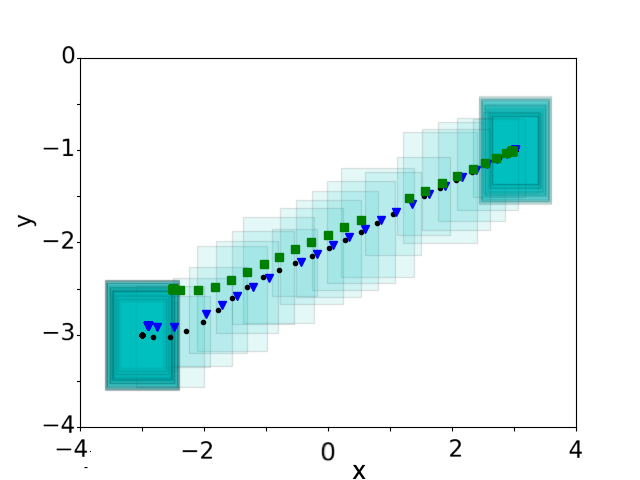
\includegraphics[width=0.4\linewidth]{figs/car_trajs.png}
    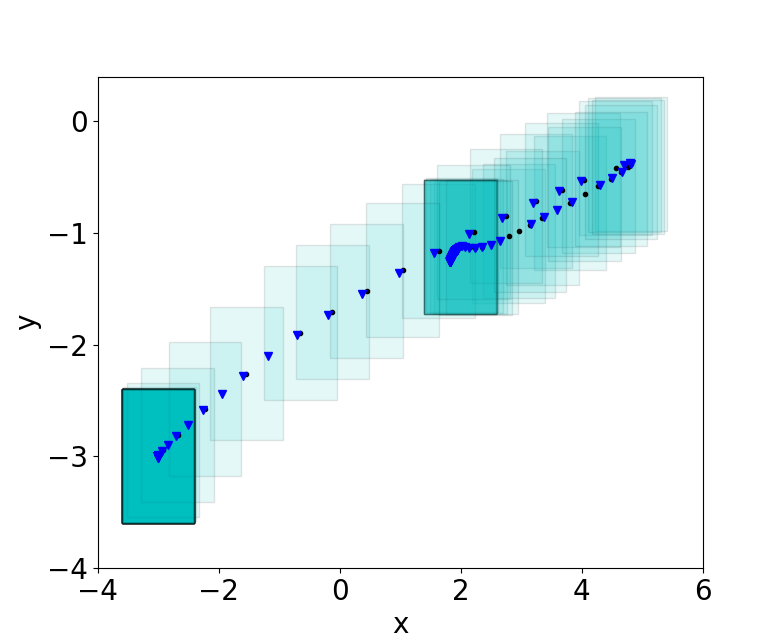
\includegraphics[width=0.4\linewidth]{figs/drone_trajs.png}
    \caption{\small \emph{Left}: Reachsets  for car. \emph{Right}: Reachtube for drone}
    \label{fig:dryVR}
\end{figure}



\newcommand{\Mposi}{\mathit{M.pos}_i}
\newcommand{\Mtgti}{\mathit{M.tgt}_i}

Following the notation in \PO{po:ind} and \PO{po:port-asm},
variables and \emph{primed copies} represents the variables in $\gconfig$, $\gconfig'$, and $\gconfig''$ respectively.

Symbolically executing the event \evname{TargetUpdate} (for robot $i$) generates the constraint:
\begin{small}
\[
E :=
\left(
\begin{array}{l}
    \neg (i = \NMAX - 1 \lor i = 0) \\
    \land\ \Mtgti' = (x[i-1] + x[i+1])/2 \land x'[i] = \Mposi \\
    \land\ \dots
\end{array}
\right)
\]
\end{small}%
Notice that it starts with the precondition and $\Mtgti$ and $x[i]$ are updated according to the effect.
The rest of formula that ensures the values of unmodified variables are unchanged
such as $\Mposi'=\Mposi$ and $x'[j]=x[j]$ for $j\neq i$, is omitted for presentation.
Additionally, a more accurate version of \asum{lineform-assume} from \refsect{overview} is
\begin{assumption}
\[
    A := \Mposi'' \in \rect(\Mposi', \Mtgti') \land \dots
\]
\end{assumption}
\noindent where the rest of the formula ensuring unchanged values is omitted.
Consequently, \PO{po:port-asm} becomes
\begin{proofob}
\[
(\forall t \in [0,\delta], \Mposi'' = f(\Mposi', \Mtgti', t)) \Rightarrow A
\]
\end{proofob}
%\chiao{Add table showing how often \PO{po:port-asm} is violated.}

The invariant for the current configuration~($\eec{\Inv}{\gconfig}$) is
\begin{small}
\[
I:= \Mposi \in \rect(x_{min}, x_{max}) \wedge x[i] \in \rect(x_{min}, x_{max})
\]
\end{small}%
and the invariant over primed configuration~($\eec{\Inv}{\gconfig''}$) is
\begin{small}
\[
I'' := \Mposi'' \in \rect(x_{min}, x_{max}) \wedge x''[i] \in \rect(x_{min}, x_{max})
\]
\end{small}%
Because there is only one event, \PO{po:ind} for \LineForm then becomes
\begin{proofob}\label{po:lineform-ind}
\(
\bigwedge\limits_{i\in \UINS} I \wedge E \wedge A \Rightarrow I''
\)
\end{proofob}

Table \ref{tab:lineform} summarizes the verification of Proof Obligation~\ref{po:lineform-ind} on systems with different $\NMAX$.

\begin{table}
    \centering
    \small
        \begin{minipage}{.25\linewidth}
            \centering
   \begin{tabular}{ |c|c @{\hspace{0.5mm}} c  c  c|  }
 \hline
       $\NMAX$&\tb{dim}  & $T_K$ (s) & $T_V$ (s)  & \tb{Safe} \\ \hline
   3   & 1 &4.90  &9.09   & \Checkmark  \\
 3   & 2 &4.19  &10.13   & \Checkmark  \\
 4    & 1 &4.79  &12.21  & \Checkmark   \\
4    & 2 &5.28  &12.49  & \Checkmark   \\
 4    & 3 &5.06  &12.77  & \Checkmark   \\
 5   & 1  &4.91  &18.46  & \Checkmark   \\
\hline
\end{tabular}
\end{minipage}
        \begin{minipage}{.28\linewidth}
            \centering
       \begin{tabular}{ c| @{\hspace{0.5mm}} c c  c  c|  }
 \hline
       $\NMAX$ &\tb{dim} & $T_K$ (s) & $T_V$ (s)  & \tb{Safe} \\ \hline
 5   & 2  &5.60  &18.91  & \Checkmark   \\
5   & 3  &5.42  &20.30  & \Checkmark   \\
10  & 1  &10.92   &32.34   & \Checkmark  \\
10  & 2  &10.96   &32.42   & \Checkmark  \\
10  & 3  &11.34   &33.61   & \Checkmark  \\
 15  & 1 &12.23  & 53.89   &\Checkmark\\
           \hline
\end{tabular}
\end{minipage}
    \caption{\small Summary of semantics based verification for \LineForm. $N$ is $\NMAX$,  $T_K$ is the symbolic post computation time in \K, $T_V$ is the time taken for construction of constraints and verification in Z3. Robots moving along a line are represented by \tb{dim} = 1, along a plane by \tb{dim} = 2, and in a 3D space by \tb{dim} = 3.}
            \label{tab:lineform}
\end{table}

Consider $\mathit{WI}$, a weaker invariant which simply constrains the position of each robot, and doesn't constrain the shared $x[i]$,
\[
\mathit{WI} := \mathit{M.pos}_i \in \mathit{rect}[x_{min}, x_{max}]
\]
Table~\ref{tab:lineform1} shows the results obtained without the proof obligations as assumptions,
and this weaker invariant on a system of robots moving in 2D. The verification procedure only tells us that the invariant is not inductive, it doesn't tell us whether the invariant doesn't hold, which is why we don't know whether the system is safe w.r.t the proposed invariant.

\begin{table}[!htbp]
    \small
 \centering
   \begin{tabular}{ |l|   c c c c|  }

 \hline
       \NMAX &\tb{constraint} & $T_K$ (s) & $T_V$ (s)   & \qquad\tb{Safe\ \ \ \ } \\ \hline
   15   & $ E\wedge I \Rightarrow I'$ & 13.06 & 23.03 & \emph{Unknown}  \\
 15   & $E \wedge \mathit{WI} \Rightarrow \mathit{WI}'$ & 9.92 & 18.26  & \emph{Unknown}  \\
 15    & $E \wedge A \wedge \mathit{WI}\Rightarrow \mathit{WI}'$ & 11.24 &  32.64 & \emph{Unknown}   \\
       \hline
\end{tabular}
    \caption{\small Verification summary for weaker invariants on \LineForm. The \tb{constraint} column displays the induction hypothesis used in the verification.  }
            \label{tab:lineform1}
\end{table}

\subsection{\Task: Distributed task allocation}
\label{sec:taskapp}

\newcommand{\ds}{\ensuremath{\epsilon}\xspace}

\Task in \reffig{taskapp} is a simple \lgname program to solve distributed task allocation problem.
The problem statement is as follows:
Given a set of (possibly heterogeneous) robots, a safety distance $\ds>0$,
and a fixed sequence of points (tasks) $\mathit{list} = x_1, x_2, \ldots \in \reals^3$,
there are following two requirements:
(a) every unvisited $x_i$ in the sequence is {\em visited\/} exactly by one robot and
(b) no two robots ever get closer than \ds.

\begin{figure}[t]

    \begin{mdframed}
        [innertopmargin=0pt,innerbottommargin=0pt]
        {%\centering
    \two{0.5}{0.5}
    {
        \lstinputlisting[language=NumKoord, lastline=22]{code/taskalloc.tex}
    }
    {
        \lstinputlisting[language=NumKoord, firstline=23, firstnumber=23]{code/taskalloc.tex}
    }}\end{mdframed}
    \caption{ $\lgname$ code for robot $i$ for the Distributed Task Allocation}
    \label{fig:taskapp}
\end{figure}

\Task consists of two events
\begin{inparaenum}[(1)]
    \item \emph{Assign}, in which each robot looks for an unassigned task $x$ from $\mathit{list}$;
    if there is a clear path to $x$ then the robot assigns itself the task $x$,
    set the actuator port $\mathit{Motion.path}$,
    and shares its path with all other robots thru $\pathvar$.
    Otherwise, it shares its position as the path.
    \item \emph{Complete}, which checks whether an robot has visited its assigned task.
\end{inparaenum}
A path here is a list of points that a robot visits in sequence.
The \Motion module drives the robot along a path,
as directed by the position value set at its actuator port $\mathit{Motion.path}$.
The sensor port $\mathit{Motion.planner}$ returns a path to the target of an unassigned task,
and a (user-defined) function called $\mathit{pathIsClear}$ is used to determine
whether the currently planned path is within \ds distance of any path in $\pathvar$.


Table \ref{tab:task} summarizes the verification of requirement~(b) for \Task with different number of robots.
\begin{table}
    \small
 \centering
   \begin{tabular}{ |l|  c c c c|  }
 \hline
 \tb{Benchmark}       & $\NMAX$ & $T_K$ (s) & $T_V$ (s)   & \qquad\tb{Safe\ \ \ \ } \\ \hline
 Task       & 3     &9.90  &10.6   & \Checkmark  \\
 Task       & 4      &9.79  &11.78  & \Checkmark   \\
 Task       & 5      &9.91  &14.92  & \Checkmark   \\
Task        & 10     &12.92   &18.34   & \Checkmark  \\
       \hline
\end{tabular}
    \caption{ \small Summary of semantics based verification for \Task.  $T_K$ is the symbolic post computation time in \K, $T_V$ is the time taken for generation of constraints and verification in Z3 and $\NMAX$ is the number of robots in the system.}
    \label{tab:task}
\end{table}

\newcommand{\DMap}{\textsf{Mapping}\xspace}
\subsection{\DMap}

The distributed grid mapping problem requires a set of robots to collaboratively mark the position of static \emph{obstacles} within a given area $D$ quantized by a \emph{grid},
which any robot should avoid while moving in $D$.
This problem is a simplified version of the distributed Simultaneous Localization and Mapping problem,
a classical problem in robotics research.
The difference comes with the assumption that the robots know their \emph{global coordinates} within the area of deployment,
and only attempt to map static obstacles within this area.
Further, the only sensors available for sensing obstacles are LIDAR based,
and the robots are constrained to move in a 2D space.

\begin{figure}[!h]
    \centering
    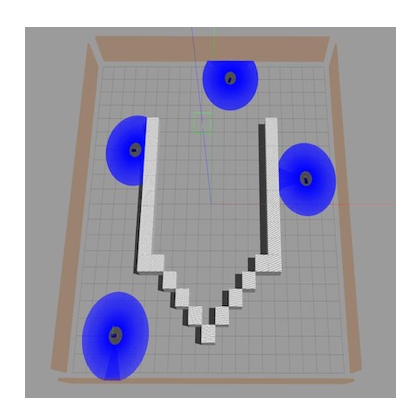
\includegraphics[scale=0.31]{figs/exp-gazebo.png}
    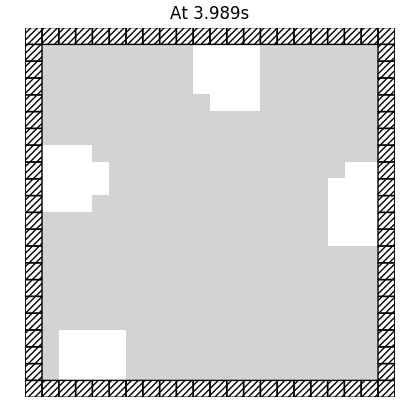
\includegraphics[width=0.21\linewidth]{figs/exp-progress-1.png}
    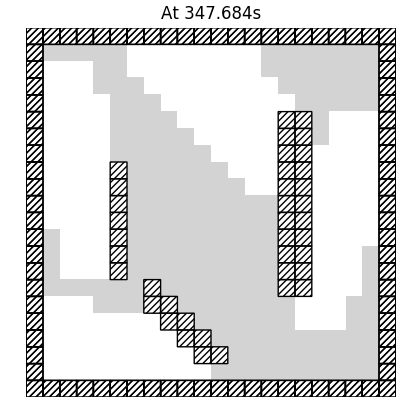
\includegraphics[width=0.21\linewidth]{figs/exp-progress-2.png}
    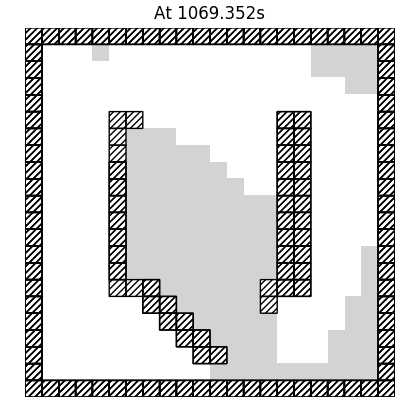
\includegraphics[width=0.21\linewidth]{figs/exp-progress-3.png}
    \caption{\small Four cars in U-shape world in simulator~(\emph{Left}). Visualization of the global map at three different time stamps~(\emph{Right})}\label{fig:U-map-progress}
\end{figure}



\begin{figure}[t]
\fbox{
    \two{0.5}{0.5}
    {\centering
        \lstinputlisting[language=NumKoord, lastline=25]{code/mapapp.tex}
    }
    {
        \lstinputlisting[language=NumKoord, firstline=26, firstnumber=26]{code/mapapp.tex}
    }
}

    \caption{\small $\lgname$ code for Distributed Mapping Application \DMap}
    \label{fig:mapapp}
\end{figure}

\newcommand{\MotionWithScan}{\emph{MotionWithScan}\xspace}
\newcommand{\chk}{\ensuremath{\mathit{chk}}\xspace}

\DMap algorithm works in the following manner.
Each robot constructs a \emph{local grid map} over $D$ using sensors,
and updates it using information from other robots shared via a \emph{global grid map}.
In \reffig{mapapp}, the \MotionWithScan module provides a $\mathit{pscan}$ sensor used to read the LIDAR scan of the actual robot.
The other sensors and actuators {\it position, reached, planner, path} have the same functionality as that in the \Motion module.
The shared allwrite variable $\gmap$ is used to construct a shared map of obstacles within the domain $D$,
and has type $\mathit{GridMap}$, which is a 2-D array representing a grid over $D$.
The local variable $\lmap$ represents each robot's \emph{local} knowledge of the domain $D$, and has the same type as $D$.
There are three \emph{events}: \emph{NewPoint, LUpdate}, and \emph{GUpdate}.
A robot executing the \emph{NewPoint} event, finds an unoccupied point to move to using a user defined function $\mathit{pickFrontierPos}$
and plans a path to it using $\mathit{MotionWithScan.planner}$.
It then updates its $\lmap$ from the shared variable $\gmap$.
The $\mathit{LUpdate}$ event updates the $\lmap$ with scanned sensor data while the robot is in motion,
and the $\mathit{GUpdate}$ event updates the shared $\gmap$ with the updated $\lmap$ information corresponding to the scanned data.

A correctness requirement for \DMap is to ensure that, at any time,
the global grid map $\gmap$ and all local maps $\lmap_i$ should be consistent with the ground truth. Table~\ref{tab:map} summarizes the verification of these constraints on systems of different $\NMAX$ .
\begin{table}
    \small
 \centering
   \begin{tabular}{ |l|  c c c c|  }
 \hline
 \tb{Benchmark}       & \tb{robots}(N) & $T_K$ (s) & $T_V$ (s)   & \qquad\tb{Safe\ \ \ \ } \\ \hline
 \dmap       & 3     &  9.23 & 14.53  & \Checkmark  \\
 \dmap      & 4      &  9.33& 19.25 & \Checkmark   \\
 \dmap       & 5      &  9.19& 24.30 & \Checkmark   \\
\dmap        & 10     &  9.31& 59.81  & \Checkmark  \\
       \hline
\end{tabular}
    \caption{ \scriptsize Summary of semantics based verification for \dmap.  $T_K$ is the symbolic post computation time in \K, $T_V$ is the time taken for generation of constraints and verification in Z3 and \emph{robots}(N) is the number of robots in the system.}\label{tab:map}
\end{table}
